The junction of \eqref{eq:chapters/11/10/4/24/L1}
    and \eqref{eq:chapters/11/10/4/24/L2} is obtained as
    \begin{align*}
	    \augvec{2}{1}{2&-3&-4\\3&4&5} \xleftrightarrow[]{R_2\rightarrow2R_2-3R_1} 
        \augvec{2}{1}{2&-3&-4\\0&17&22} \\
		      \xleftrightarrow[]{R_1\rightarrow17R_1+3R_2} \augvec{2}{1}{17&0&-1\\0&17&22} 
		      \implies
        \vec{A} = \frac{1}{17}\myvec{-1\\22}
    \end{align*}
    Clearly, the man should follow the path perpendicular to \eqref{eq:chapters/11/10/4/24/L3} from
    $\vec{A}$ to reach it in the shortest time. The normal vector 
    of \eqref{eq:chapters/11/10/4/24/L3} is 
    \begin{align}
         \myvec{6\\-7}
	 \implies
        \vec{n} = \myvec{7\\6}
        \label{eq:chapters/11/10/4/24/L4-norm}
    \end{align}
    and the equation of the desired line is
   \begin{align}
        \myvec{7&6}\vec{x} &= \frac{1}{17}\myvec{7&6}\myvec{-1\\22} = \frac{125}{17}
        \label{eq:chapters/11/10/4/24/L4}
    \end{align}
		See Fig. \ref{fig:chapters/11/10/4/24/crossing}.
		\begin{figure}[H]
        \centering
        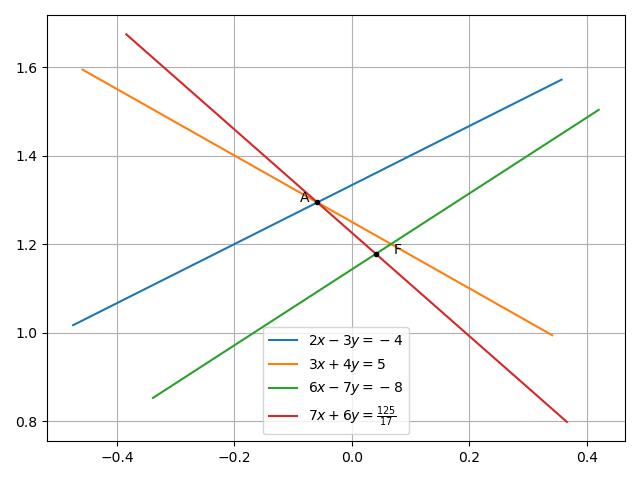
\includegraphics[width=0.75\columnwidth]{chapters/11/10/4/24/figs/crossing.png}
        \caption{AF is the required line.}
        \label{fig:chapters/11/10/4/24/crossing}
    \end{figure}
